\subsection{豪斯多夫商空间}

我们来寻求使商空间 X/R 为豪斯多夫空间的条件（这时称等价关系 R 为豪斯多夫的）。首先，若 X/R 是豪斯多夫的，则 X/R 中由单点组成的诸子集是闭的（第 1 目，命题 4），因而每个模 R 的等价类在 X 中是闭的。但这个必要条件并不充分。

X/R 中开集的定义给出如下的必要充分条件：X/R 是豪斯多夫的，当且仅当 X 中任意两个不同的等价类都包含在 X 的两个不相交的饱和开子集中。我们将给出其他更便于使用的条件。

命题 8. 商空间 X/R 为豪斯多夫的一个必要条件是 R 的图象 C 在 X × X 中是闭的。若等价关系 R 是开的，则此条件也是充分的。

设 \(\varphi: X \to X/R\) 是典范映射；则 \(C\) 是 \(\varphi \times \varphi: X \times X \to (X/R) \times (X/R)\) 下对角线 \(\Delta\)（即 \((X/R) \times (X/R)\) 的对角线）的逆像。因此命题的第一部分由 \(\varphi \times \varphi\) 的连续性得出{[}公理 \((H^{ii})\) 及 §2 第 1 目定理 1{]}。若 \(R\) 是开的，则 \((X/R) \times (X/R)\) 可等同于商空间 \((X \times X)/(R \times R)\)（§5，第 3 目，命题 8 的推论），而 \(\Delta\) 这时等同于 \((X \times X)/(R \times R)\) 中集合 \(C\)（它关于 \(R \times R\) 是饱和的）的典范象。于是 \(\Delta\) 在 \(X \times X\) 中是闭的，从而 \(X\) 是豪斯多夫的。

\pandocbounded{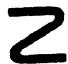
\includegraphics[keepaspectratio]{images/part001_7b053cb2.jpg}}

若 R 不是开的，则存在这样的例子：C 是闭的而 R 不是豪斯多夫的（习题 10 与 28）。

为证 X/R 是豪斯多夫的，我们也可以应用第 1 目命题 5：设 M 与 N 是 R 的两个不同的等价类，只需存在 X 的一个开子集 A 到豪斯多夫空间 \(X'\) 中的一个连续映射 f，其中 A 关于 R 饱和且包含 M 与 N，使得 1) f 在 A 所含的每个模 R 等价类上取常值，2) f 在 M 与 N 上取不同的值。因为既然 \(A/R_{A}\) 可等同于 X/R 的一个开子集（§ 3，第 6 目，命题 10，推论 1），我们就可以对由 f 诱导的映射 g: \(A/R_{A} \to X'\) 应用第 1 目命题 5，因为 g 是连续的（§ 3，第 4 目，命题 6）。

特别地：

命题 9. 若 \(f\) 是拓扑空间 \(\mathbf{X}\) 到豪斯多夫空间 \(\mathbf{X}'\) 中的一个连续映射，而 \(\mathbf{R}\) 是等价关系 \(f(x) = f(y)\)，则商空间 \(\mathbf{X} / \mathbf{R}\) 是豪斯多夫的。

命题 10. 若 X 是豪斯多夫空间，且 X 关于等价关系 R 有一个连续截面 s，则 X/R 是豪斯多夫的，且 s (X/R) 在 X 中是闭的。

因为（§ 3，第 5 目）X/R 同胚于 X 的子空间 \(s(\mathrm{X}/\mathrm{R})\)，后者是豪斯多夫的。此外，\(s(\mathrm{X}/\mathrm{R})\) 是由所有 \(x \in \mathbf{X}\) 中使 \(s(\varphi(x)) = x\) 的点组成的集合，其中 \(\varphi: \mathbf{X} \to \mathbf{X}/\mathbf{R}\) 是典范映射；因此第二个断言由第 1 目命题 2 得出。

